\documentclass{IEEEcsmag}

\usepackage[colorlinks,urlcolor=blue,linkcolor=blue,citecolor=blue]{hyperref}
\expandafter\def\expandafter\UrlBreaks\expandafter{\UrlBreaks\do\/\do\*\do\-\do\~\do\'\do\"\do\-}
\usepackage{upmath,color}
\usepackage{graphicx}
\usepackage{booktabs}

\jvol{XX}
\jnum{XX}
\paper{8}
\jmonth{Month}
\jname{Computing in Science \& Engineering}
\jtitle{Computing in Science \& Engineering}
\pubyear{2026}

\setcounter{secnumdepth}{0}

\begin{document}

\sptitle{Feature Article: Research Practice}

\title{Managing the Research Process, Not Only Its Outputs: Fifteen Requirements and How to Meet Them}

\author{Telmo Miguel-Medina}
\affil{Electromechanical Engineering Department, University of Burgos, Burgos, 09001, Spain}

\markboth{FEATURE ARTICLE}{FEATURE ARTICLE}

\begin{abstract}\looseness-1
Research infrastructure has concentrated on stewarding outputs: data, software, publications. This article asks what it takes to manage the process that produces them. A bibliometric map of 5{,}139 works and a review of 88 studies show attention concentrated on data management and analysis (51\% and 42\% of the corpus) and falling to 3.7\% for the formulation of ideas and questions. Tracing documented challenges to management needs yields fifteen tool-independent requirements, each with checkable capabilities. Three (research planning, research-question management and decision traceability) are highly important yet weakly served; in a test on 36 further reviews, none addressed the last two. For each requirement I give a minimum practice and an observable check, ordered into three adoption tiers: record, coordinate, connect and release. The result is a checklist for research groups and students, and explicit criteria for evaluating research tools.
\end{abstract}

\maketitle

\chapteri{A} modern research project is not a single artifact but a chain of them: a question, a protocol, a literature corpus, data, analysis code, a computational environment, intermediate results, figures, a manuscript, and eventually released software and supplementary material. These objects evolve continuously, are touched by distributed and often multidisciplinary teams, and computational and data-intensive research keeps adding more of them while raising the cost of keeping them consistent.\textsuperscript{1}

In everyday practice, these artifacts and the work that produces them are scattered across disconnected systems: email, cloud drives, spreadsheets, reference managers, statistical software, code repositories, task boards, manuscript editors. Each tool serves its own purpose well, but the layer that should coordinate them is largely missing. Reviews of research data management and of post-award grant management repeatedly link this fragmentation to weak decision traceability, incomplete process documentation, inconsistent versioning and low project visibility.\textsuperscript{2,3}

Two decades of work on scientific workflow systems, provenance, research data management and open-science platforms have produced solid evidence on stewarding research \emph{outputs}: repositories, persistent identifiers, curation, dissemination.\textsuperscript{1,2} Managing the research \emph{process} (planning, question formulation, decision tracking, cross-stage coordination) has received far less attention. The review literature is itself split into strands that each stop short of it. Workflow surveys start from an executable pipeline and take the question and the plan behind it as given.\textsuperscript{1} Provenance research tracks the lineage of data and computation but rarely reaches the upstream intellectual choices.\textsuperscript{4,5} Data-management reviews center on data as an output, and the lifecycle models they rely on have been criticized for presenting research as linear and purposive.\textsuperscript{2,6} Research-information-system reviews are pitched at institutional reporting,\textsuperscript{7} and open-science syntheses at outputs and their dissemination.\textsuperscript{8}

The distinction matters for the quality of research. A result whose question, plan and analytic decisions cannot be reconstructed cannot be audited, however well its data and code are archived. Reviews of provenance in biomedicine and of open geographic science both report that reproducibility is more often a stated ideal than a demonstrated, end-to-end achievement, and that leaving documentation until dissemination leaves most projects irreproducible.\textsuperscript{4,5,9}

None of these strands says what a research group would need in order to manage the process as a whole. Requirements appear in this literature only implicitly, as challenges listed at the end of a review, scattered across fields with different vocabularies. This article makes them explicit. It asks three questions. Which stages of the research lifecycle does the literature under-serve? What requirements for managing a research project follow from the challenges the literature documents? And what minimum practices meet those requirements, whatever tools a group happens to use? The answer to the last question is deliberately tool-independent: which platforms satisfy the requirements, and how well, is a separate evaluation that I report elsewhere.

\section{HOW I STUDIED THIS}

I used two instruments on the same topic, one broad and shallow, one narrow and deep.

The first is a bibliometric map. Fifteen title-and-abstract queries against OpenAlex, covering research-process management, data management and open science, version control in research, and virtual research environments, filtered to 2008--2025 and complemented by five arXiv queries, produced 5{,}139 works after de-duplication. Two checks bound its quality: a sampled precision estimate of 0.94 for the four broadest queries, and an independent Scopus and Web of Science search that shares only 22\% of its DOIs with the corpus but whose non-overlapping records are mostly tool papers that mention ``workflow'' in passing. Each work's abstract and index terms were then matched against a lexicon of eleven \emph{lifecycle themes}, four or five terms per theme. A work counts toward every theme it matches, so the shares do not sum to 100\%. Because simple substring matching over-counts short terms (``doi'' inside ``doing''), I recomputed the profile with word-anchored matching as a sensitivity check.

The second is a review of the secondary literature, with studies identified by two routes. The first route was an AI-assisted literature search (Consensus Deep Search), which screened candidates with a machine-learned relevance filter; the 52 studies its synthesis cites, 41 of them secondary syntheses, formed the initial evidence base. Because that screening is not open to inspection, and because only 21 of those 52 studies turned out to be in my own corpus, I added a second, fully reproducible route: a systematic screen of the corpus itself. A title filter for secondary-study designs (review, survey, mapping study, bibliometric analysis and similar) reduced the 5{,}139 works to 291 candidates. Each was screened on title and abstract against written criteria: it had to be a secondary study, and it had to concern infrastructure or practice for managing the research process or its artifacts. Of the 291, 109 were not secondary studies (questionnaire surveys, protocols, tool papers), 130 were off topic, five dealt only with technical internals such as scheduling, and two were duplicate versions. Forty-five were eligible: nine already in the evidence base and 36 new. The review therefore covers 88 studies.

I used the two sets differently. The first 52 were coded by literature strand and lifecycle focus, and from them I rated the attention the literature gives to each of fifteen \emph{lifecycle stages}, a finer list than the eleven themes, as heavy, moderate or thin. The 36 new studies were held back as a test set for the requirements, as described below.

Requirements were derived from the first 52 studies, through an explicit chain. A \emph{challenge} is a problem that one or more studies report about how research is currently managed. A \emph{need} restates it as what a research group lacks. A \emph{derived requirement} states what a system or practice must provide. This produced seventeen derived requirements. Reconciling them with a provisional list of fourteen domains drafted beforehand broadened three domains and added one, giving fifteen requirements, RM1 to RM15. Twelve of the seventeen rows map one-to-one, two requirements absorb two rows each, and the last row (governance) became the fifteenth requirement.

Each requirement carries a definition; three to six \emph{expected capabilities}, the observable things a system or practice must do for the requirement to count as met; a three-tier rating of \emph{literature attention} (weak: addressed incidentally or only named as a gap; moderate: addressed by some strands but not across the lifecycle; strong: recurring across reviews with mature tooling); an ordinal \emph{importance} rating based on the weight of evidence and on how many other requirements depend on it; and its dependencies. Attention measures coverage, not importance. A requirement that is highly important but appears in the literature only as a named gap is a \emph{differentiator}.

I was the only human coder. As a consistency check, a large language model independently assigned the seventeen rows to the fifteen definitions and agreed on sixteen (Cohen's $\kappa$ = 0.94); this tests agreement with the written definitions, not expert judgment. The same model applied the written screening criteria to the 291 candidates and coded the 36 new studies; every decision, with its reason, is published.

To test whether the requirement set holds beyond the studies it was built from, the challenge reported in the abstract of each of the 36 new studies was mapped to the fifteen requirements, recording any challenge that fitted none. Finally, for each requirement I wrote the least a research group can do to realize its capabilities, with a check that the practice is in place, and ordered these by dependency. The full query strings, the list of 88 studies, the screening decisions, the row-by-row derivation with its sources, and every script are in the public study repository (see Acknowledgments).

\section{WHERE THE LITERATURE LOOKS}

The literature is an assembly of partly connected strands rather than one field. Annual output in the corpus rises from 60 works in 2008 to 585 in 2024, nearly tenfold, led by venues in digital curation, distributed computing and the life sciences. The keyword map (Figure~\ref{fig:coword}) shows workflow, provenance and research data management as the terms that bridge otherwise separate clusters. Among the first 52 reviewed studies, workflow systems are the largest strand (13), followed by research information systems (10) and provenance (7); 22 studies address execution and only three address the upstream stages.

\begin{figure}[t]
\centerline{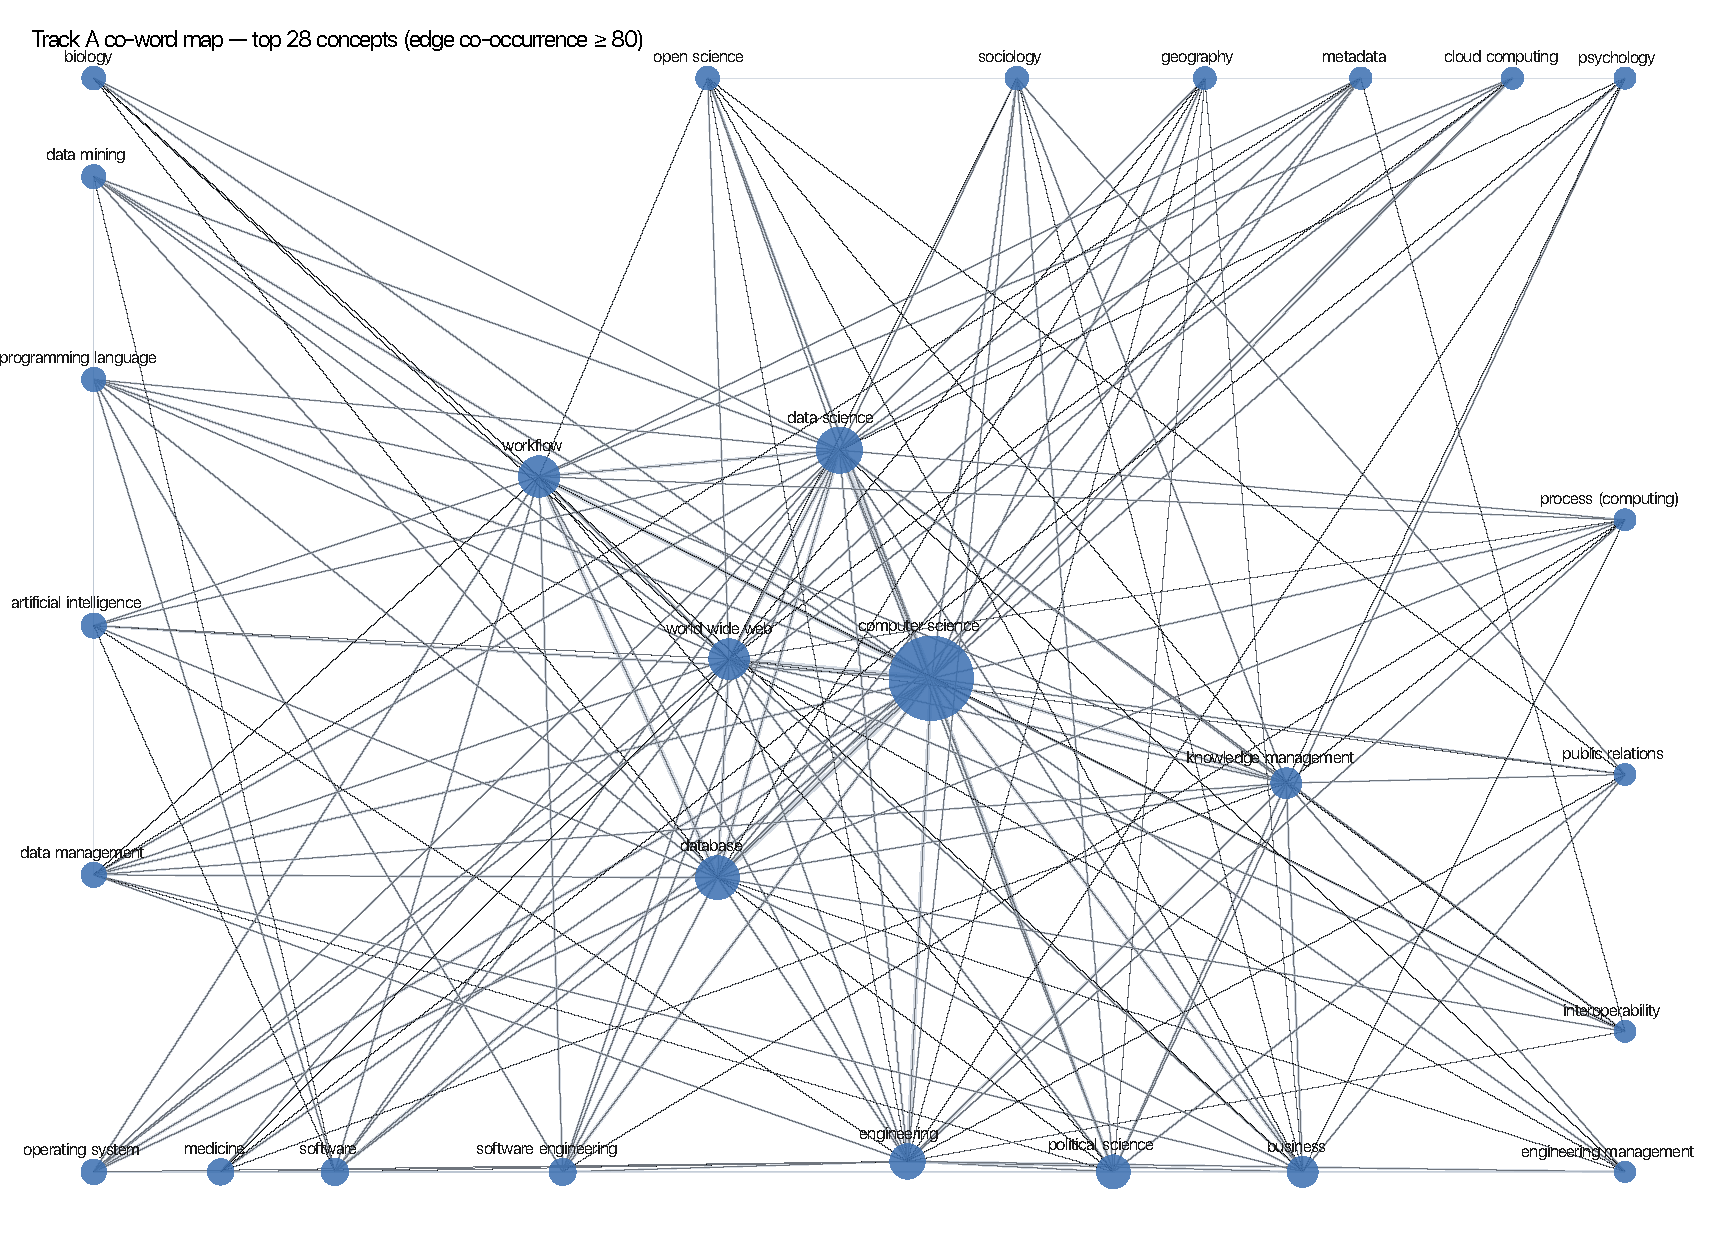
\includegraphics[width=18.5pc]{coword_map.pdf}}
\caption{Keyword co-occurrence map of the 5{,}139-work corpus. Workflow, provenance and research data management bridge the clusters; the upstream stages of the research process are largely absent.}\label{fig:coword}
\end{figure}

Attention across the lifecycle is markedly uneven (Table~\ref{tab:themes}). Data management and analysis dominate, matched by 50.8\% and 41.9\% of the corpus. Dissemination and coordination follow at 23.5\% and 21.1\%. Idea and question formulation comes last, at 3.7\%. Under the stricter matching rule only one theme moves by more than a percentage point, and both ends of the ranking stay where they are.

\begin{table}[t]
\caption{Share of the 5{,}139-work corpus matching each lifecycle theme, under substring matching and under word-anchored matching. Themes are not mutually exclusive.}\label{tab:themes}
\tablefont
\begin{tabular*}{17.5pc}{@{\extracolsep{\fill}}lrr@{}}
\toprule
Theme& Substring (\%)& Anchored (\%)\\
\colrule
Data management& 50.8& 50.8\\
Analysis and workflow& 41.9& 41.9\\
Dissemination& 23.5& 23.4\\
Coordination& 21.1& 21.1\\
Methods and protocol& 13.7& 13.7\\
Planning& 12.5& 11.8\\
Literature& 9.9& 9.8\\
Outputs and identification& 9.8& 5.6\\
Governance& 8.9& 8.9\\
Provenance& 7.0& 7.0\\
Idea and question& 3.7& 3.7\\
\botrule
\end{tabular*}
\end{table}

The close reading agrees. Of fifteen lifecycle stages, the reading of the first 52 studies rates seven as thinly covered: idea generation, research-question refinement, planning, ethics review, post-publication traceability, cross-stage coordination, and governance. Four are heavily covered, all concerned with data, analysis and outputs, and provenance is heavily studied but incomplete, concentrated on data and computation rather than upstream decisions.\textsuperscript{4,5}

The two instruments agree on the extremes and diverge on one point. A fifth of the corpus matches the coordination theme, yet the review rates coordination as thin. The difference is one of granularity: the lexicon catches any mention of collaboration, while the review asks about lifecycle-wide coordination infrastructure, which it finds only in domain-specific forms. The common pattern is that the literature is strongest where research can be formalized as data pipelines, repository transactions or institutional information flows, and weakest where the thing to be managed is the evolving process itself.

Three explanations fit the evidence. Computational experiments can be expressed as executable graphs, so they attract taxonomies and repeated surveys;\textsuperscript{1} a research question that is reformulated twice during a project has no comparable formal object. Lifecycle models present research as linear, masking iteration and tacit judgment,\textsuperscript{6} so infrastructure designed from them begins where data begins.\textsuperscript{2} And outputs are what repositories, identifiers and research information systems are built to count.\textsuperscript{7,8} Recent work on AI-supported planning shows growing interest upstream, but it remains thin.\textsuperscript{10}

\section{FIFTEEN REQUIREMENTS}

Table~\ref{tab:requirements} gives the fifteen requirements, each next to the documented challenge it answers. They fall into nine categories. Traceability is the largest, with four (research-question management, decision traceability, version control, provenance and artifact linkage), followed by documentation with three (documentation, transparency, reproducibility support) and collaboration with two. Eight requirements are rated of high importance. The evidence is concentrated: one scoping review of research data management supports four requirements,\textsuperscript{2} and one of biomedical provenance supports three.\textsuperscript{4}

\begin{table*}[t]
\caption{The fifteen research-management requirements, the documented challenge each one answers, and how well the reviewed literature covers it. $^\star$ marks a differentiator: high importance, but present in the literature only as a named gap. ``New'' is the number of the 36 held-back studies whose reported challenge maps to the requirement. Row-by-row sources are in the study repository.}\label{tab:requirements}
\tablefont
\setlength{\tabcolsep}{4pt}
\begin{tabular*}{\textwidth}{@{\extracolsep{\fill}}p{22pt}p{104pt}<{\raggedright}p{186pt}<{\raggedright}p{38pt}p{54pt}r@{}}
\toprule
ID& Requirement& Documented challenge it answers& Attention& Importance& New\\
\colrule
RM1$^\star$& Research planning and roadmap& Planning and early phases are under-represented; infrastructure starts at data& Weak& High& 2\\
RM2$^\star$& Research-question management& Question refinement is rarely supported or documented& Weak& High& 0\\
RM3& Task management& Coordination relies on ad hoc scripts and spreadsheets& Weak& High& 3\\
RM4& Documentation& Scripts and workflows are poorly documented; documentation is deferred to dissemination& Strong& High& 2\\
RM5$^\star$& Decision traceability& Upstream intellectual decisions are not captured by provenance tools& Weak& High& 0\\
RM6& Collaboration and contribution tracking& Informal coordination is invisible; contributions are not attributed& Moderate& Medium-high& 1\\
RM7& Communication& Multisite and collaborative work is hard to align& Moderate& Medium& 2\\
RM8& Version control& Data standards, analyses and manuscripts evolve without traceable versions& Moderate& High& 4\\
RM9& Artifact management and integration& Fragmented tools and custom scripts break continuity between stages& Strong& High& 4\\
RM10& Provenance and artifact linkage& Provenance coverage is incomplete; papers, tools, data and code are disconnected& Strong& High& 6\\
RM11& Transparency& The research process is opaque to third parties& Weak& Medium-high& 1\\
RM12& Reproducibility support& Reproducibility is treated as a design ideal, not demonstrated end to end& Strong& Medium-high& 3\\
RM13& Automation& Testing and metadata validation are manual and inconsistent& Moderate& Medium& 2\\
RM14& Output management and identification& Outputs are not linked to the activities that produced them; metadata standards are incompatible& Strong& Medium-high& 9\\
RM15& Governance and sustainability& Long-term services, funding and workforce are weakly addressed& Weak& Low-medium& 9\\
\botrule
\end{tabular*}
\end{table*}

Attention and importance are not aligned. On the first reading, the literature covers five requirements strongly, four moderately and six weakly. Three of the weakly covered ones are rated highly important while the literature offers no more than a statement of the gap: research planning (RM1), research-question management (RM2) and decision traceability (RM5). These differentiators sit at exactly the stages both instruments found thinnest. I keep them at full strength for that reason: the absence of literature on a need is not evidence that the need is small.

The 36 held-back studies test this picture (last column of Table~\ref{tab:requirements}). Twenty-eight report a challenge in their abstract, and 27 of those map to at least one existing requirement. The test supports the differentiators more sharply than I expected: not one of the 36 reviews addresses research-question management or decision traceability, and only two address planning. It also corrects the framework in two places. Governance and sustainability, which I had rated as weakly covered, is one of the two most frequent concerns in the new set (nine studies, mostly from library and data-management reviews reporting missing policy, funding and skills), so its attention rating should be read as strong at the institutional level. And one theme has no proper home: three reviews concern access control and privacy for sensitive data, which the framework touches only through the access policy listed under governance.

What makes a requirement usable is its expected capabilities. Decision traceability, for instance, is met when a decision can be recorded with its rationale and the alternatives considered, timestamped, attributed to the people who took it, and linked to the artifacts it affects. Research-question management is met when a question can be registered, its revisions kept, and the methods, analyses and outputs that address it linked to it. A tool, or a group's working practice, can be checked against each capability in turn, and the evidence for each judgment shown, so that a reader can see why a rating was given and disagree with it. That is the intended use of the framework, and the reason it was derived without reference to any platform.

The requirements also depend on one another, and the dependencies matter for what comes next. Two are substrates: documentation underlies decision traceability, provenance, transparency and reproducibility support, and version control underlies collaboration, provenance and output management. Two are consumers: provenance draws on questions, documentation, decisions, versions and organized artifacts, because an end-to-end chain cannot be retrieved unless each link was recorded; and transparency is not a separate capability but what results when the others are inspectable. Governance, whose institutional side (ownership continuity, funding, workforce) no project can settle alone, frames them all.\textsuperscript{11}

\section{WHAT TO DO ABOUT IT}

Table~\ref{tab:recs} states, for each requirement, the least a research group can do to meet it and how to tell that it has. None of the practices presupposes a tool: a decision log can live in a text file, a wiki or an issue tracker. The dependencies give them an order.

\begin{table*}[t]
\caption{A minimum, tool-independent practice and an observable check for each requirement, by adoption tier.}\label{tab:recs}
\tablefont
\setlength{\tabcolsep}{4pt}
\begin{tabular*}{\textwidth}{@{\extracolsep{\fill}}p{22pt}p{232pt}<{\raggedright}p{186pt}<{\raggedright}@{}}
\toprule
Req.& Minimum practice& Check\\
\colrule
\multicolumn{3}{@{}l}{\emph{Tier 1: record}}\\
RM4& Keep the project description, methods and protocol as versioned plain-text documents, started before data collection& A dated methods document predates the first data or analysis file\\
RM8& Put every text-based artifact under one version history; name the version behind anything reported; record identifiers or checksums for artifacts held elsewhere& Any reported result can be tied to one named version\\
RM5& Keep a numbered decision log: date, context, decision, alternatives, rationale, artifacts affected& Every change of question, method, inclusion criterion or analysis plan has an entry\\
RM2& Give each research question an identifier; revise by appending, never overwriting; cite the identifier from methods, analyses and manuscript& Each reported result names the question it answers\\[3pt]
\multicolumn{3}{@{}l}{\emph{Tier 2: coordinate}}\\
RM1& Maintain one plan of record (phases, objectives, milestones); log each revision as a decision& The current plan and its earlier versions can both be retrieved\\
RM3& Keep one task list with owner, status and priority; link each task to what it produced& Each completed task points to an artifact or a decision\\
RM6& Have a second person review substantive changes before they are integrated; record who contributed what& Contributions are attributable; review comments are preserved\\
RM7& Move agreements out of email and chat into threaded records linked to the task or artifact concerned& A newcomer can find why a task exists without asking\\
RM9& Document a directory layout with one home per artifact type; point to external artifacts with location, version and access conditions& Every artifact named in the manuscript can be located from the project root\\[3pt]
\multicolumn{3}{@{}l}{\emph{Tier 3: connect and release}}\\
RM10& Make every change reference the task, question or decision behind it; record the script and data version behind every figure and table& From any result, the chain back to its question can be followed without the author\\
RM11& Publish a status summary and change log readable without privileged access; state what is embargoed and until when& A third party can tell what has been done and what changed\\
RM12& Record the environment and pinned versions; provide one documented entry point that regenerates the results& A clean run reproduces the reported tables\\
RM13& Automate the checks that are otherwise skipped: structure validation, link checking, regeneration of tables and figures& The checks run without anyone remembering to run them\\
RM14& Release named versions; deposit each where it receives a persistent identifier; ship machine-readable citation metadata& Each cited version resolves to an archived copy\\
RM15& Name an owner; write down the access policy, the contribution rules and where the record goes when the project ends& The project survives the departure of any one person\\
\botrule
\end{tabular*}
\end{table*}

\emph{Record first.} Start with the two substrates and the two upstream records that depend only on them: documentation written from the first day, version control of every text-based artifact, a decision log, and a register of research questions. Everything later consumes these, a single researcher can adopt them alone, and two of the three differentiators are here. Keeping track of how results were produced and putting everything under version control is established advice for computational work.\textsuperscript{12} What the requirements add is that the same discipline applies to questions and decisions, not only to code and data.

\emph{Then coordinate.} Add the practices whose value depends on there being a plan and more than one person: a plan of record whose revisions are logged as decisions, a single task list linked to outputs, review before integration, communication moved into linked and searchable records, and a documented layout for artifacts.

\emph{Then connect and release.} The remaining practices consume the earlier ones: linking every change and every result to the question, decision and task behind it; making status and history inspectable; capturing what is needed to re-derive the results; automating the checks that are otherwise forgotten; releasing identified, citable versions; and settling ownership, access and exit.

For a student or a new group member, the checks in Table~\ref{tab:recs} are the practical part. Experienced researchers know, without stating it, that a change of inclusion criterion needs a recorded reason, and that a figure should be traceable to the script and data version that made it. A beginner has to learn this by imitation unless someone writes it down. Each check is a question a supervisor can ask and a student can answer with evidence.

Two other audiences can use the same material. For tool builders, the differentiators show where first-class objects are missing: a research question with a revision history and typed links to the methods and results that address it; a decision with its alternatives and affected artifacts; a plan whose revisions are retrievable. For journals, funders and reviewers, the checks suggest what could be asked of a submission beyond data and code availability, in particular a decision log and a question register, the two records that make the path from question to result auditable.

\section{WHAT THIS MEANS, AND WHAT IT DOES NOT}

Two independent readings of the literature, one counting themes across five thousand works and one reading the review literature closely, place its attention on the part of research that produces files and its neglect on the part that produces decisions. The requirements derived from that literature inherit the pattern. What research infrastructure lacks is not another repository or identifier scheme but support for the deliberative, upstream process.

It would overstate the evidence to say that managing the process improves research quality. Much of the reviewed literature is descriptive or self-reported, with little empirical evaluation of whether any given infrastructure improves quality, traceability or coordination.\textsuperscript{2} The narrower claim the evidence supports is that an unrecorded process cannot be assessed. Where the question, the plan and the analytic decisions are recorded with their reasons, a reader can tell a planned analysis from a post hoc one, and a justified deviation from an unexplained one. The requirements are conditions for auditing rigor, not a guarantee of it.

Several limitations bound these findings. The requirements were derived from 52 studies found by an AI-assisted search whose screening is not transparent; the systematic screen that tests them is reproducible, but it finds secondary studies only by the design named in their title, and it codes abstracts, not full texts. Screening and test coding were done by a language model under written criteria, and I was the only human coder; the attention and importance ratings were not independently re-coded. Primary studies are outside the review altogether. The requirement set was reconciled with a provisional list, so it is not purely inductive, although every requirement is backed by at least one extracted challenge. The evidence is concentrated in biomedicine, computer science and library and information science, in English, and a few reviews support several requirements each. The theme profile is coarse: 9.5\% of works match no theme and three lifecycle stages have none, so its value lies in the ranking, which is stable, not in the individual percentages. And the recommendations are derived, not tested: the tier order is a hypothesis about adoption, not an observed result.

The next steps follow from these. Full-text extraction from the 36 new reviews, a second human screener, and an extension to primary studies would show whether the requirement set is stable beyond review abstracts, and whether handling sensitive data deserves a requirement of its own. An expert panel across disciplines should replace my single judgment on importance. And applying the expected capabilities as explicit criteria to the platforms research groups already use would show which requirements current tooling meets and which it leaves to convention.

\section{CONCLUSION}

The literature on research infrastructure is output-biased. Half of a 5{,}139-work corpus concerns data management, and fewer than four works in a hundred concern the formulation of ideas and questions; in a close reading of the review literature, seven of fifteen lifecycle stages are thinly covered, and they are the upstream and cross-cutting ones. Tracing the challenges this literature documents to management needs yields fifteen tool-independent requirements, each with capabilities that can be checked. Three of them (research planning, research-question management and decision traceability) are highly important and weakly served (of 36 further reviews used as a test, none addresses the last two), and they mark where new tooling and new reporting expectations would do the most good. Because the requirements depend on one another, they can be adopted in order: record first, then coordinate, then connect and release. The framework does not prescribe a tool. It states what any tool, and any research group, should be able to show.

\section{ACKNOWLEDGMENTS}
The study repository (bibliographic corpus, the list of reviewed studies, screening decisions, coding sheets, the row-by-row requirement derivation with its sources, and every script) is openly available at \url{https://github.com/telmomm/github-research-infrastructure-study} and archived on Zenodo, DOI \href{https://doi.org/10.5281/zenodo.22167500}{10.5281/zenodo.22167500}, with a companion dataset record at DOI \href{https://doi.org/10.5281/zenodo.22173525}{10.5281/zenodo.22173525}. The author declares no competing interests and received no specific funding.

\def\refname{REFERENCES}

\begin{thebibliography}{1}

\bibitem{liew2016}
C. S. Liew, M. P. Atkinson, M. Galea, T. F. Ang, P. Martin, and J. I. van Hemert, ``Scientific workflows: Moving across paradigms,'' {\it ACM Comput. Surveys}, vol. 49, no. 4, pp. 1--39, 2016.

\bibitem{perrier2017}
L. Perrier et al., ``Research data management in academic institutions: A scoping review,'' {\it PLoS ONE}, vol. 12, no. 5, p. e0178261, 2017.

\bibitem{crane2023}
K. Crane, A. Blatch-Jones, and K. Fackrell, ``The post-award effort of managing and reporting on funded research: A scoping review,'' {\it F1000Research}, vol. 12, p. 863, 2023.

\bibitem{gierend2024}
K. Gierend et al., ``Provenance information for biomedical data and workflows: Scoping review,'' {\it J. Med. Internet Res.}, vol. 26, 2024, doi: 10.2196/51297.

\bibitem{johns2023}
M. Johns et al., ``Data provenance in biomedical research: Scoping review,'' {\it J. Med. Internet Res.}, vol. 25, 2023, doi: 10.2196/42289.

\bibitem{cox2018}
A. Cox and W. Tam, ``A critical analysis of lifecycle models of the research process and research data management,'' {\it Aslib J. Inf. Manage.}, vol. 70, no. 2, pp. 142--157, 2018.

\bibitem{haris2026}
M. Haris, S. Auer, and M. Stocker, ``Research information systems and knowledge graphs: A review,'' {\it Front. Res. Metrics Anal.}, vol. 11, p. 1786866, 2026.

\bibitem{klebel2025}
T. Klebel, V. Traag, I. Grypari, L. Stoy, and T. Ross-Hellauer, ``The academic impact of Open Science: A scoping review,'' {\it R. Soc. Open Sci.}, vol. 12, no. 3, p. 241248, 2025.

\bibitem{holler2022}
J. Holler and P. Kedron, ``Mainstreaming metadata into research workflows to advance reproducibility and open geographic information science,'' {\it Int. Arch. Photogramm. Remote Sens. Spatial Inf. Sci.}, vol. XLVIII-4/W1-2022, pp. 201--208, 2022.

\bibitem{devkota2026}
N. Devkota, M. Siddique, D. Karki, and D. Thapa, ``Research in the age of AI---How to plan? A bibliometric exploration of the research lifecycle,'' {\it Int. Res. J. MMC}, vol. 7, no. 3, pp. 94--116, 2026.

\bibitem{donner2022}
E. K. Donner, ``Research data management systems and the organization of universities and research institutes: A systematic literature review,'' {\it J. Librarianship Inf. Sci.}, vol. 55, no. 2, pp. 261--281, 2022.

\bibitem{wilson2017}
G. Wilson, J. Bryan, K. Cranston, J. Kitzes, L. Nederbragt, and T. K. Teal, ``Good enough practices in scientific computing,'' {\it PLoS Comput. Biol.}, vol. 13, no. 6, p. e1005510, 2017.

\end{thebibliography}

\begin{IEEEbiography}{Telmo Miguel-Medina}{\,}is with the Electromechanical Engineering Department, University of Burgos, Burgos, 09001, Spain. His research interests include research software engineering, open science infrastructure and reproducible computational research. Contact him at tmiguel@ubu.es.
\end{IEEEbiography}

\end{document}
